\input{config}

\begin{document}
 \newpage
\ESKDthisStyle{empty}

\begin{center}
Министерство образования и науки Российской Федерации\\
Федеральное государственное бюджетное образовательное учреждение высшего профессионального образования\\
ТОМСКИЙ ГОСУДАРСТВЕННЫЙ УНИВЕРСИТЕТ СИСТЕМ УПРАВЛЕНИЯ И РАДИОЭЛЕКТРОНИКИ (ТУСУР)\\
Кафедра комплексной информационной безопасности электронно-вычислительных систем (КИБЭВС)\\
\end{center}

\vspace{2cm}

\begin{center}
Отчет по преддипломной практике \\
на тему \\
``Механизм взаимодействия датчиков и центрального сервера АСКУЭ''
\end{center}

\vspace{2cm}

\begin{flushright}
Выполнил: \\
студент гр. 720-1 \\
\underline{\hspace{2.5cm}}Д.С. Никифоров \\
"\underline{\hspace{1cm}}"\underline{\hspace{3cm}} 2015г.\\
\end{flushright}

\begin{flushright}
Утвердил: \\
директор ЦСП ТУСУР: \\
\underline{\hspace{2.5cm}}А.А. Конев \\
"\underline{\hspace{1cm}}"\underline{\hspace{3cm}} 2015г.\\
\end{flushright}

\vfill
\begin{center}
Томск -- 2015
\end{center}
 \newpage
\ESKDthisStyle{empty}
\paragraph*{\hfill РЕФЕРАТ \hfill}
Отчет по преддипломной практике содержит \ESKDtotal{page} страниц, \ESKDtotal{figure} рисунка, \ESKDtotal{bibitem} источников. % \ESKDtotal{table} таблицы, \ESKDtotal{appendix} приложение.

АСКУЭ, ПРОТОКОЛ, СВЯЗЬ, СЕРВЕР, TCP/IP, УСПД.

Цель работы -- выбор протокола вхаимодействия между сервером и устройствами сбора данных АСКУЭ.

В ходе работы был сделан обзор существующих протоколов.

Пояснительная записка выполнена при помощи системы компьютерной вёрстки \LaTeX.
 \newpage
\ESKDthisStyle{empty}
\paragraph*{\hfill THE ABSTRACT \hfill}

Diploma work contains \ESKDtotal{page} pages, \ESKDtotal{figure} pictures, 19 tables, \ESKDtotal{bibitem} sources, \ESKDtotal{appendix} appendix, 5 sheets of a graphic material.

ASCEA, PROTOCOL, LINK, SERVER, TCP/IP, QT, NETWORK.

Purpose -- to create a protocol interaction between the data acquisition server (DAS) and removal and data transmission devices (RDTD) in an automated system of commercial accounting of energy resources (ASCAE).

The work included a review of existing protocols, sensor interaction with the server; highlighted threats to the information transmitted through the communication channels between the DAS and the RDTD, the mechanisms of protection against threats, developed the communication protocol and the RDTD DAS, emulators implemented RDTD DAS testing protocol, launched and testing protocol. 

An explanatory note is made by means of computer typesetting \LaTeX.
 \newpage
\ESKDthisStyle{empty}

\begin{center}
Министерство образования и науки Российской Федерации\\
Федеральное государственное бюджетное образовательное учреждение высшего профессионального образования\\
ТОМСКИЙ ГОСУДАРСТВЕННЫЙ УНИВЕРСИТЕТ СИСТЕМ УПРАВЛЕНИЯ И РАДИОЭЛЕКТРОНИКИ (ТУСУР)\\
Кафедра комплексной информационной безопасности электронно-вычислительных систем (КИБЭВС)\\
\end{center}

\begin{flushright}
 \begin{minipage}{0.4\textwidth}
  УТВЕРЖДАЮ \\
  Зав. кафедры КИБЭВС \\
  \underline{\hspace{2.5cm}}А.А. Шелупанов \\
  "\underline{\hspace{1cm}}"\underline{\hspace{3cm}} 2015г.
 \end{minipage}
\end{flushright}

\vspace{2cm}

\begin{center}
 ЗАДАНИЕ \\
% На преддипломную практику
\end{center}

Студенту Дмитрию Сергеевичу Никифорову группы 720-1, факультета безопасности.

% 1. Тема преддипломной практики: ``Механизм взаимодействия датчиков и центрального сервера АСКУЭ''
% 
% 2. Исходные данные к проекту: Документация к проекту разработки АСКУЭ.
% 
% Руководитель практики: \\ директор ЦСП ТУСУР Антон Александрович Конев. 
% 
% \hfill Подпись руководителя: \underline{\hspace{2.5cm}}
% 
% \hfill "\underline{\hspace{1cm}}"\underline{\hspace{3cm}} 2015г.
% 
% Задание принял к исполнению
% 
% Студент гр. 720-1 Дмитрий Сергеевич Никифоров \hfill \underline{\hspace{2.5cm}}
% 
% \hfill "\underline{\hspace{1cm}}"\underline{\hspace{3cm}} 2015г.
 \newpage
 \tableofcontents
 \vspace{1cm}
 \begin{minipage}[left]{0.6\linewidth}
  Компакт диск: \\
  Пояснительная записка в формате PDF
 \end{minipage}
 \hfill
 \begin{minipage}[right]{0.3\linewidth}
  В конверте на обороте обложки 
 \end{minipage}
 
 \vspace{1cm}
 
 \begin{minipage}[left]{0.6\linewidth}
  Графический материал \\ (демонстрационные листы):
 \end{minipage}
 \hfill
 \begin{minipage}[right]{0.3\linewidth}
  На отдельных листах
 \end{minipage}
 
 \vspace{1cm}
 
 Плакат 1
 
 Плакат 2
 
 Плакат 3
 
 Плакат 4
 
 Плакат 5 Технико-экономическое обоснование
 
 \newpage

\section*{Введение}
\addcontentsline{toc}{section}{Введение}

Основными  потребителями  электросчетчиков российского производства являются страны СНГ, Украина и Казахстан – лидеры по потреблению в 2007-2013 году (на долю экспорта в эти страны приходится около  80\% \cite{rbk} ),  поэтому,  в  данном  обзоре  рассмотрены  наиболее распространенные АСКУЭ представленные на рынках России, Казахстана, Украины и Белоруссии.


Целью данной работы является определить наиболее популярные протоколы передачи данных, поддерживаемые в приборах и системах учета, с целью их анализа, выбора и дальнейшей реализации в разрабатываемой автоматизированной гетерогенной системе коммерческого учета энергоресурсов.
 \newpage
\section{Описание разрабатываемой автоматизированной системы коммерческого учета энергоресурсов}
\setcounter{figure}{0}

Основными  потребителями  электросчетчиков российского производства являются страны СНГ, Украина и Казахстан – лидеры по потреблению в 2007-2013 году (на долю экспорта в эти страны приходится около  80\% [1] ). Для учета использования электроэнергии существуют автоматизированные системы коммерческого учета электроэнергии (АСКУЭ).

Автоматизированная система коммерческого учета энергоресурсов (АСКУЭ) - это программно-аппаратный комплекс, предназначенный для сбора, хранени и обработки инофрмации о потреблении энергоресурсов на объекте. 

Аппаратная часть представлена устройствами учета(УУ), устройствами сбора и передачи данных(УСПД), а так же центральным сервером(ЦС).

Программная часть включает в себя прошивки УУ и УСПД, ПО для ЦС.

ПО ЦС предназначено для сбора показаний с точек учета энергоресурсов, а также архивирования, хранения, анализа и визуализации полученных данных, формирования отчетов. Под показаниями подразумеваются данные о потребляемой мощности электроэнергии потребителями однофазных и трехфазных сетей.

Областью применения ПО ЦС являются объекты жилого, коммерческого и производственного назначения.

ПО ЦС — это программный комплекс, который должен включать в себя сервер баз данных, сервер сбора данных(ССД), сервер приложений, web-сервер, АРМ оператора, АРМ администратора, АРМ клиента, АРМ сервисного инженера.

ПО ССД должно выполнять следующие функции:
\begin{itemize}
 \item взаимодействие с УСПД и счетчиками (опрос и сбор данных);
 \item взаимодействие с СБД (запись обработанных данных для дальнейшей работы с ними);
 \item преобразование полученных данных в удобный для дальнейшей обработки формат;
 \item мониторинг и обработка ошибок;
 \item журналирование событий ССД.
\end{itemize}

ПО ЦС представляет собой иерархическую систему сбора, передачи и хранения данных (рис. \ref{irsh:irsh}). Информация от первичных приборов учета посредством УСПД поступает на ССД, который обеспечивает ее обработку и запись на СБД.

\begin{figure}[h!]
 \center{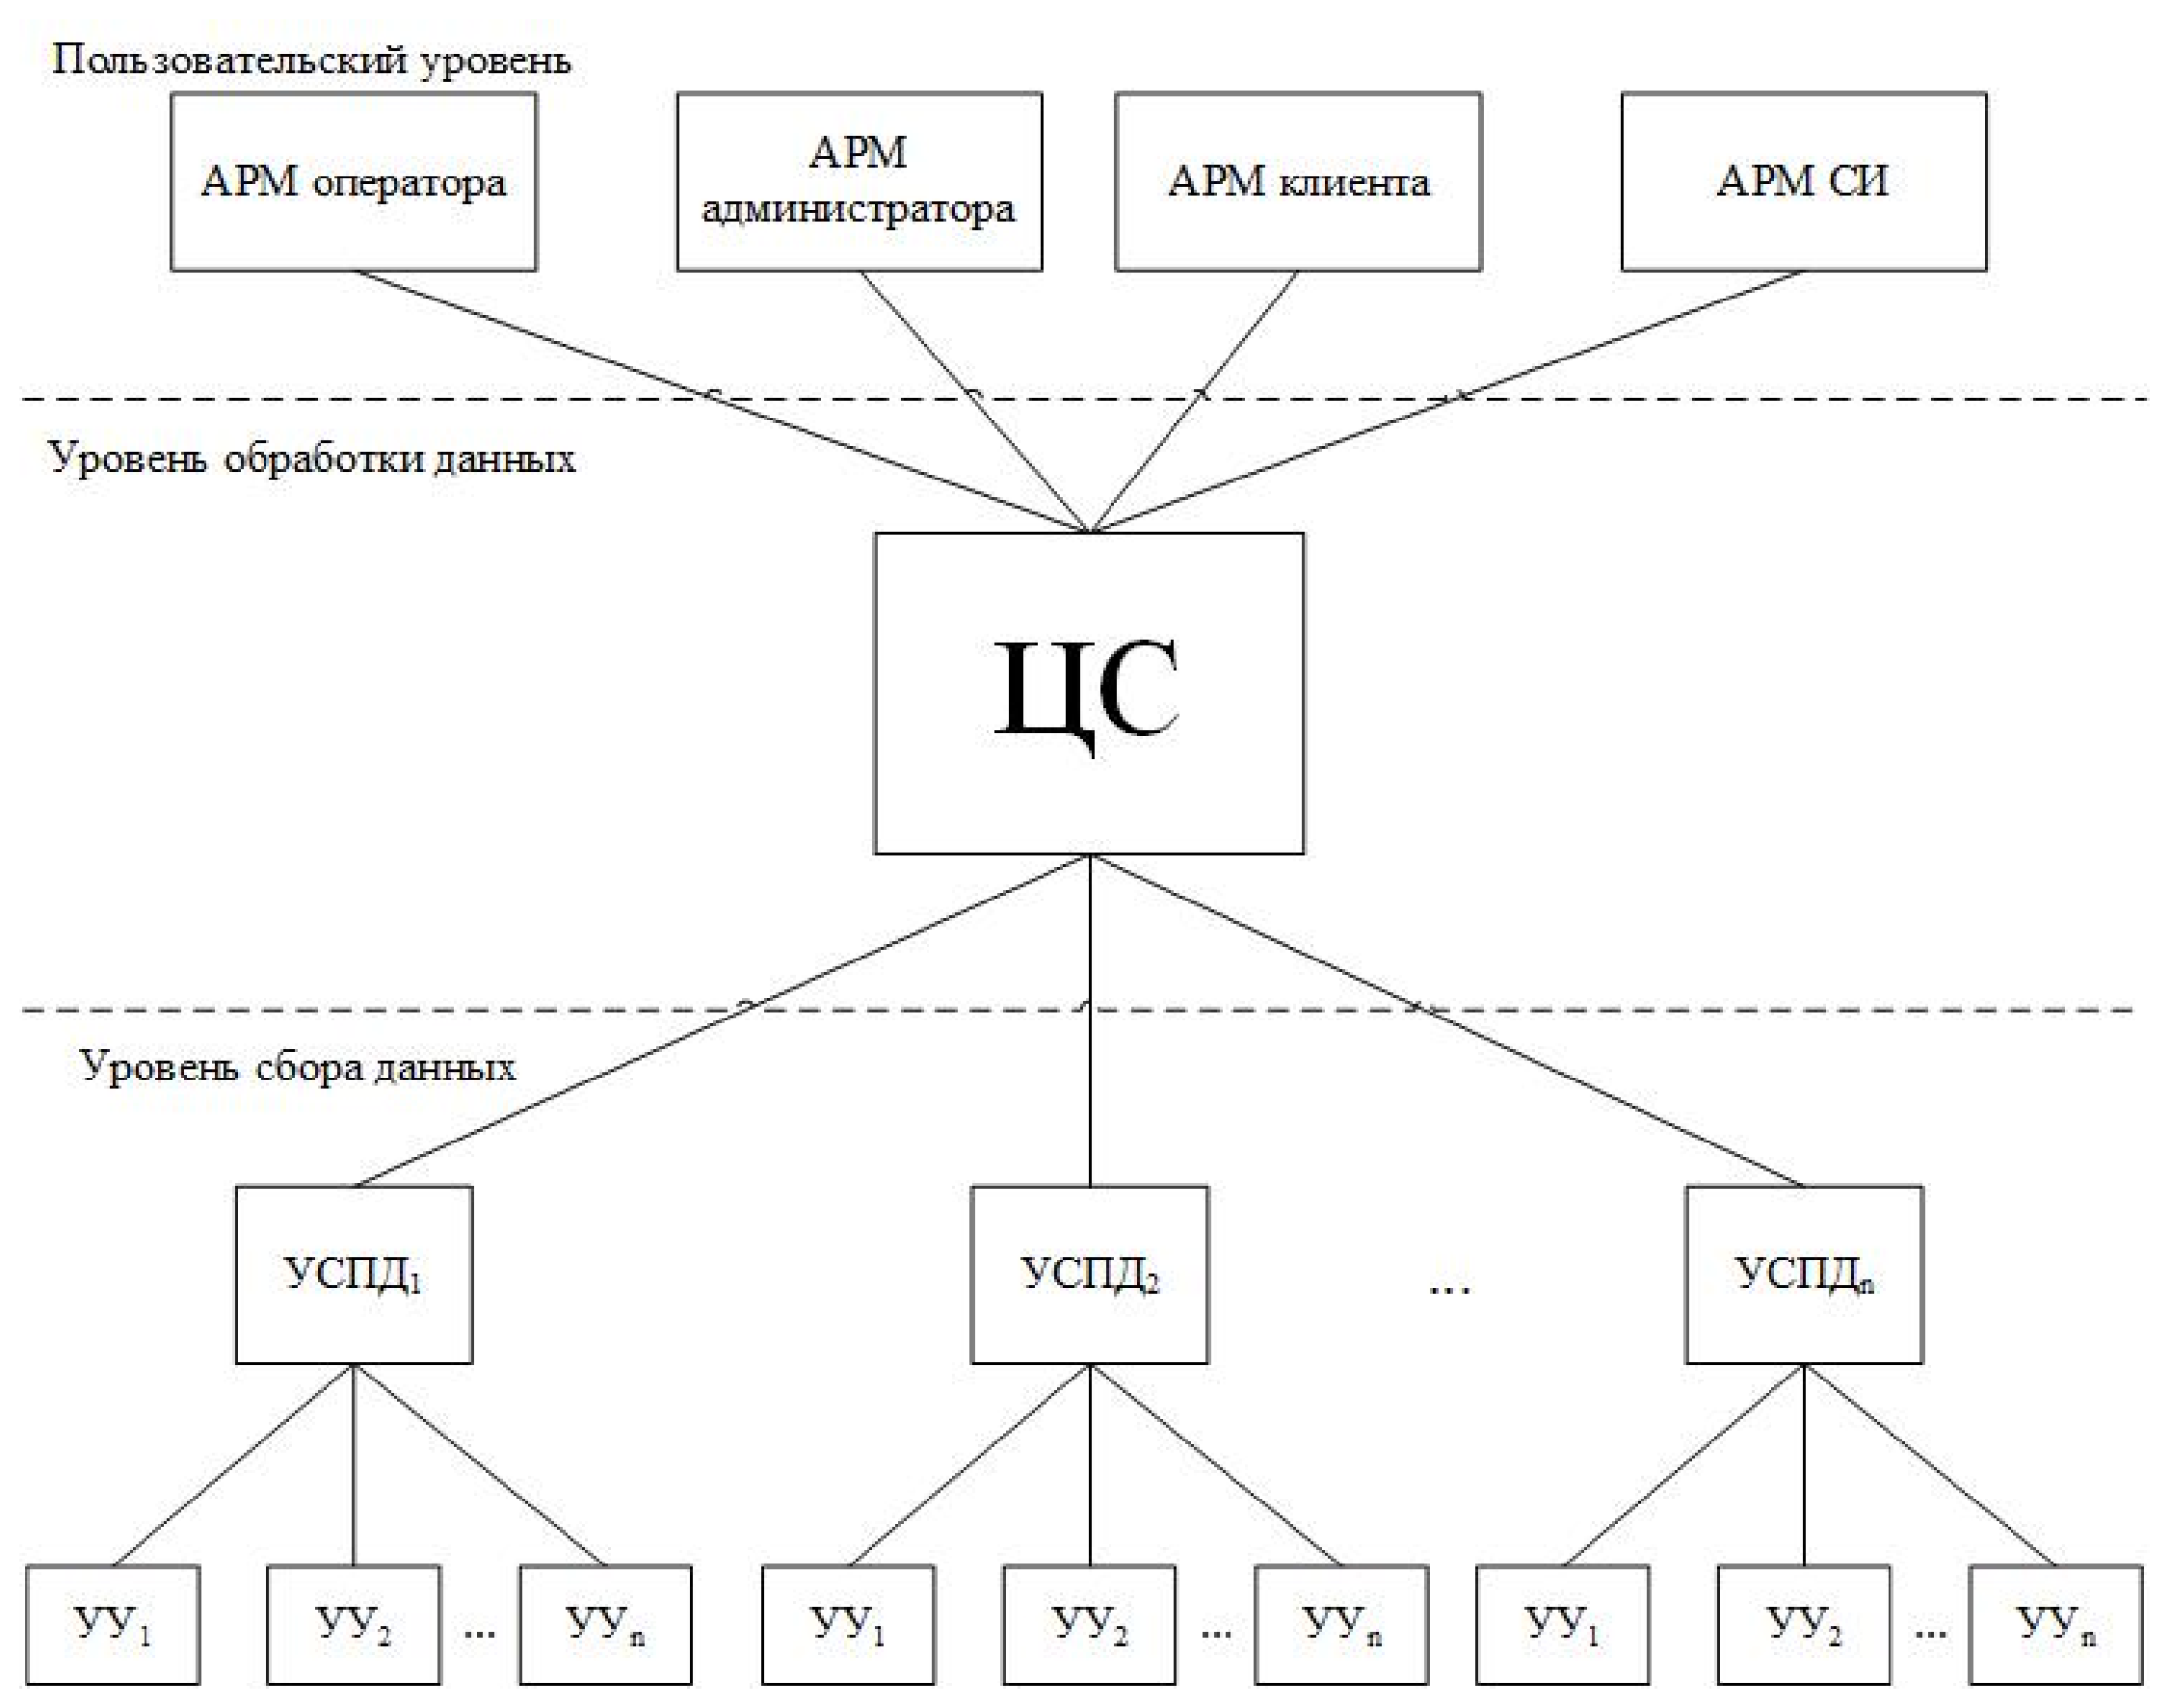
\includegraphics[width=0.8\linewidth]{irsh}}
 \caption{Структурная схема АСКУЭ}
 \label{irsh:irsh}
\end{figure}

\subsection{Описание сервера сбора данных}

ССД обслуживает низкоуровневое взаимодействие с УСПД. После получения данных этот блок передает информацию модульной системе драйверов. Система драйверов осуществляет взаимодействие на верхнем уровне модели OSI. За счет модульности обеспечивается расширение парка поддерживаемого оборудования. Также ССД содержит систему управления сетью и взаимодействия с базой данных: он осуществляет контроль работоспособности сети, выполняет отбраковку данных, отвечает за принятие решений о повторном запросе на сбор данных, классифицирует информацию, обеспечивает контроль единого времени и осуществляет запись информации в базу данных.

Логически ПО ССД можно разделить на 3 блока, каждый из которых выполняет отдельную задачу:
\begin{enumerate}
\item блок контроля приема и передачи данных, который отвечает за взаимодействие ССД с УСПД/УУ;
\item временная база данных (ВБД). В ходе проектирования ПО ССД было рассмотрено два варианта обработки и записи данных с УСПД/УУ на СБД: 
\begin{itemize}
\item обработка и запись данных на СБД по мере их поступления от УСПД/УУ;
\item запись поступающих данных в ВБД и последующая обработка и передача на СБД.
\end{itemize}
\item блок обработки данных.
\end{enumerate}

Использование первого варианта может привести к потере данных, так как вновь поступающие данные не будут успевать обрабатываться ПО ССД. Второй вариант позволяет обеспечить целостность поступивших данных, поэтому он является более предпочтительным.

Обобщенная функциональная схема функционирования ПО ССД представлена на рисунке \ref{sh_ssd:sh_ssd}.

\begin{figure}[h!]
 \center{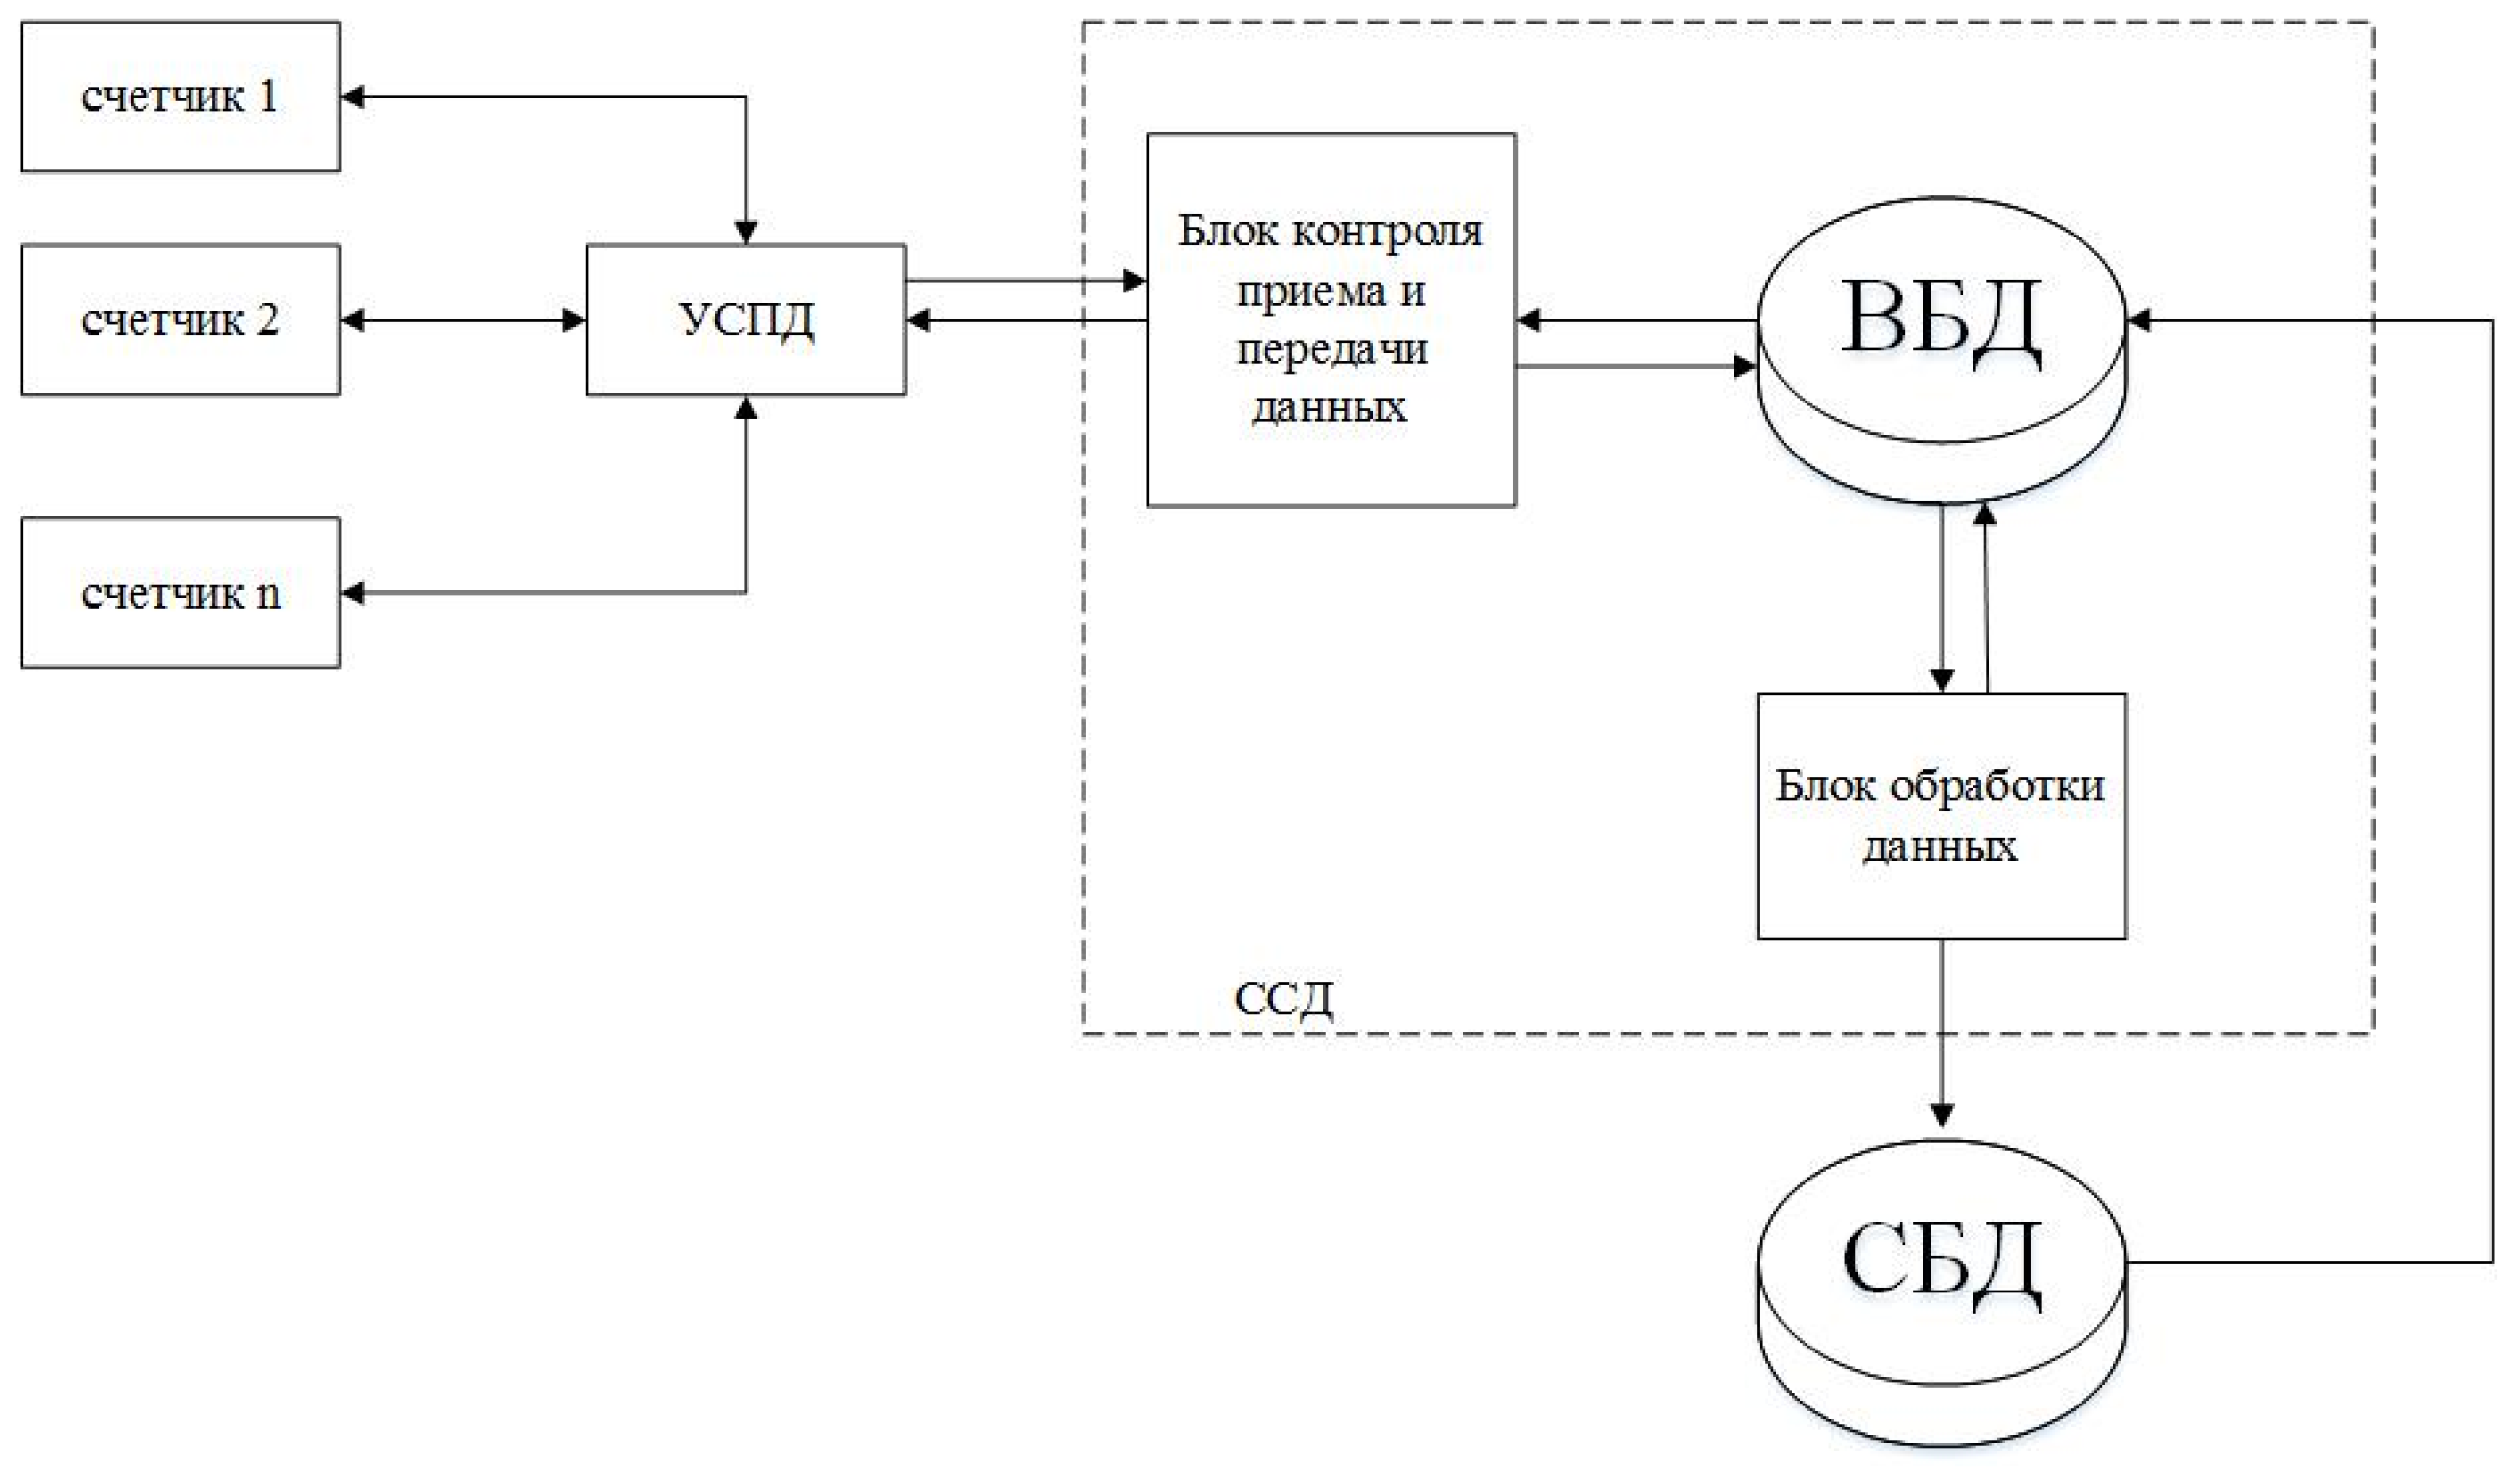
\includegraphics[width=0.8\linewidth]{sh_ssd}}
 \caption{Функциональная схема ССД}
 \label{sh_ssd:sh_ssd}
\end{figure}

\subsection{Описание устройства съема и передачи данных}

Устройство съема и передачи данных является промежуточным звеном между устройствами учета и сервером сбора данных. Оно предназначено для непосредственного управления устройствами учета, их опроса, настройки и диагностики. Всю инофрмацию от устройств учета и о их состоянии ССД получает от УСПД.

%TODO мало написано про УСПД %описание ССД и УСПД, тут же требования к взаимодействию??? 
 \newpage
\section{Входные и выходные данные}
\setcounter{figure}{0}

\subsection{Входные данные}
Для осуществления сбора показаний ССД необходимо получить от ЦБД список подконтрольных ему УСПД. Так же на ССД должны находиться данные для идентификации и аутентификации на УСПД. 

Списком УСПД является набор строк, которые содержат в себе идентификатор УСПД и его IP-адрес, по которому он доступен в сети интернет. 

Данными для идентификации и аутентификации являются закрытые ключи шифрования и пары ``имя пользователя'' и ``пароль''.

%TODO имхо маловато для описаия входных данных. добавить формат хотя бы для списка УСПД.

\subsection{Выходные данные}

По запросу ССД получает от УСПД пакет данных который содержит показания УУ, информацию о состоянии УУ и информацию о состоянии УСПД. Структура данного покета представлена на рисунке \ref{img:answer_struct}.

\begin{figure}[!ht]
 \center{
\includegraphics[width=0.8\linewidth]{answer_struct}}
 \caption{Структура пакета, получаемого от УСПД}
 \label{img:answer_struct}
\end{figure}

Пакет состоит из пяти блоков:

\begin{enumerate}
 \item идентификатор УСПД - уникальная для каждого УСПД последовательность из 2 байт, позволяющая однозначно идентифицировать УСПД;
 \item размер блока УСПД - размер в байтах блока данных о УСПД (4 байта);
 \item блок информации о состоянии УСПД - информация о состоянии УСПД, текущее времени на УСПД;
 \item блок данных УУ - размер в байтах блока данных о УУ (4 байта);
 \item блок информации от УУ - последовательность структур данных, содержащих информацию о каждом УУ, подконтрольном УСПД и показания данного УУ.
\end{enumerate}

Структура данных, содержащая информацию о каждом УУ представлена на рисунке \ref{img:UU_struct}.

\begin{figure}[!ht]
 \center{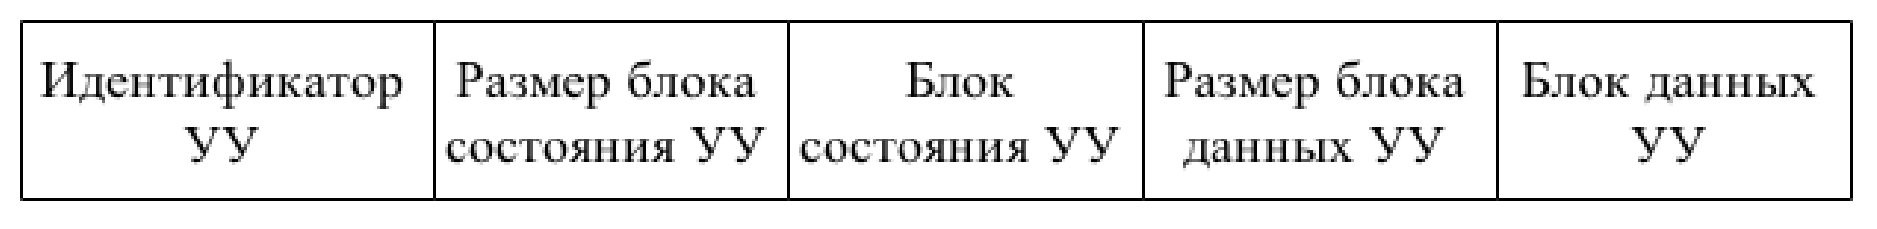
\includegraphics[width=0.8\linewidth]{UU_struct}}
 \caption{Структура данных, получаемая от УУ}
 \label{img:UU_struct}
\end{figure}

Структура состоит из пяти блоков:

\begin{itemize}
 \item идентификатор УУ - уникальный для каждого УУ байт, позволяющий однозначно идентифицировать УУ подконтрольный указанному УСПД;
 \item размер блока состояния УУ - размер в байтах блока информации о состоянии УУ;
 \item блок состояния УУ - блок данных о состоянии УУ;
 \item размер блока данных УУ - размер в байтах блока данных, собранных УУ;
 \item блок данных УУ - данные, собранные прибором учета.
\end{itemize}
 % описание входных и выходных данных
 \section{Используемые протоколы}
\setcounter{figure}{0}

На рынке представлено множество датчиков, которые связываються с системой по различным протоколам. Используются такие протоколы как [2]:
\begin{itemize}
\item TCP/IP;
\item Modbus;
\item Canbus;
\item МЭК 60870-5-101;
\item МЭК 60870-5-104;
\item ОРС;
\item "Пирамида" (закрытый протокол);
\item спецпротоколы электросчетчиков;
\item SNMP;
\item TFTP;
\item RTU-325.
\end{itemize}

\subsection{Стандарт OPC}

OPC (OLE for Process Control) – семейство протоколов,предоставляющих единый интерфейс для управления объектами автоматизации и технологическими процессами. В частности, OPC DA (DataAccess) — стандарт, описывающий набор функций обмена данными в реальном времени с объектами автоматизации. 

Спецификация OPC охватывает:
\begin{itemize}
 \item концепцию клиент-серверную технологию OPC и определение данных;
 \item описания интерфейсов, методов, параметров и возможное ихповедение;
 \item описание типов и структур данных;
 \item общие виды деятельности, которые включают в себя определениеадресного пространства и егопросмотра. Чтение, запись и подписка науведомления об обновлении данных.
\end{itemize}

К недостаткам этого OPC можно отнести:
\begin{itemize}
 \item необходимость платного членствавсообществе The InteroperabilityStandard for Industrial Automation;
 \item протокол основан на технологиях windows.
\end{itemize}

\subsection{Стандарт МЭК-60870-5-101/104}

МЭК-60870-5-101/104 – это протокол передачи данных, применяется в АСКТУ, АСКУЭ. Особенности реализации протокола МЭК 60870-101/104 при передаче данных между объектом и диспетчерским центром:

\begin{itemize}
 \item передача ограниченного количества информации, что обусловлено необходимостью переназначения всех сигналов с одного протокола на другой, и, как следствие, потеря некоторых данных, передача которых на этапе проектирования не была сочтена целесообразной;
 \item отсутствие единых наименований сигналов в рамках объекта и в центрах управления сетями, приводящее к сложности наладки и отслеживания ошибок;
 \item протокол МЭК 60870-5-101 предназначен для передачи данных по последовательным линиям связи RS-232/485;
 \item протокол МЭК 60870-5-104 является расширением протокола 101 и регламентирует использование сетевого доступа по протоколу TCP/IP.
\end{itemize}

Недостатки реалищации данного стандарта:

\begin{itemize}
 \item количество передаваемых сигналов ограничивается определенным количеством дискретных входов и выходов;
 \item отсутствует возможность контроля связи между устройствами;
 \item возможно ложное срабатывание дискретного входа устройства при замыкании на землю в цепи передачи сигнала;
 \item цепи подвержены воздействию электромагнитных помех;
 \item сложность расширения систем;
 \item передача данных осуществляется в два этапа:
 \begin{enumerate}
  \item назначение индексированных коммуникационных объектов на прикладные объекты;
  \item  назначение прикладных объектов на переменные в прикладной базе данных или программе. Таким образом, отсутствует семантическая связь (полностью или частично) между передаваемыми данными и объектами данных прикладных функций.
 \end{enumerate}
 \item протоколы не предусматривают возможность передачи сигналов реального времени.
\end{itemize}

\subsection{Стандарт MODBUS}

Modbus – один из наиболее распространенных сетевых протоколов для интеграции устройств РЗА (релейная защита автоматики) в систему АСТУ, построенный на архитектуре «клиент–сервер». Данный протокол является открытым, что частично обуславливает его популярность. Протокол Modbus для передачи данных использует такие линиям связи как RS-485, RS-433, RS-232, а также сети TCP/IP (Modbus TCP).

Стандарт Modbus содержит в себе:

\begin{itemize}
 \item спецификация прикладного уровня;
 \item спецификация канального уровня;
 \item спецификация физического уровня;
 \item спецификацию ADU для транспорта через стек TCP/IP.
\end{itemize}

К достоинствам стандарта относится:

\begin{itemize}
 \item массовость;
 \item относительная простота реализации систем на его базе.
\end{itemize}

К недостаткам данного протокола можно отнести:

\begin{itemize}
 \item в случае необходимости отсутствует возможность оперативной сигнализации от конечного устройства к мастеру;
 \item стандарт не регламентирует начальную инициализацию системы. Назначение сетевых адресов и параметров системы для каждого устройства выполняются вручную на этапе адаптации;
 \item отсутствие  возможности  конечным  устройствам  обмениваться фиксированными данными друг с другом без участия мастера. Что ограничивает  применимость MODBUS-решений в системах регулирования реального времени.
\end{itemize}

\subsection{Стандарт CAN}

CAN (Controller Area Network) – стандарт промышленной сети, использующийся для объединения в единую сеть устройств и датчиков. Применяется в системах автоматизации промышленного производства. 

В первую очередь данный стандарт описывает физический уровень, наибольшую популярность получил вариант описанный в ISO 11898-2. Физический уровень использует дифференциальную передачу данных по витой паре, для управления доступом к шине используется неразрушающее bit-wise разрешение конфликтов ISO 11898.

К положительным аспектам данной реализации относиться:

\begin{itemize}
 \item работа в режиме жёсткого реального времени;
 \item высокая устойчивость к помехам;
 \item надёжный контроль ошибок приема-передачи данных.
\end{itemize}

К достоинствам данного стандарта относятся:

\begin{itemize}
 \item сообщения имеют малые размеры (8 байт данных) и защищены контрольной суммой;
 \item большой размер служебных данных в пакете по отношению к полезным данным;
 \item отсутствие единого общепринятого стандарта на протокол высокого уровня.
\end{itemize}

\subsection{Стандарт DLMS}

DLMS (Device Language Message Specification) – стек протоколов, ориентированный на 16-разрядные микроконтроллеры Microchip PIC. Является международным стандартом для систем сбора данных с электро-, газовых, водяных и тепловых счетчиков. Работает на основе протоколов связи (RS232, RS485, PSTN, GSM, GPRS, IPv4, PPP и PLC), с поддержкой шифрования AES128.

Особенности данного протокола:

\begin{itemize}
 \item работает на всех 16-битных микроконтроллерах PIC и dsPIC;
 \item возможность интеграции стека DLMS с текущими реализациями протоколов TCP/IP, ZigBee и PLC;
 \item небольшой объем занимаемой памяти позволяет использовать компактные и недорогие контроллеры;
 \item для европейского рынка стек поддерживает IEC 62056-21 Mode E.
\end{itemize}

К недостаткам данного протокола можно отнести то, что описание протокола предоставляется на платной основе или требуется членство в ассоциации DLMS.

Из представленного краткого анализа видно, что существующие протоколы связи достаточно успешно позволяют реализовывать задачи диспетчерского управления / интеграции данных в системы управления, однако не все они позволяют реализовывать функции реального времени. К тому же большое количество проприетарных протоколов приводит к усложнению процесса интеграции устройств в единую систему: 
\begin{itemize}
 \item протоколы должны поддерживаться контроллером и ЦППС, что требует реализации поддержки большого количества протоколов в УСО и ЦППС одновременно и ведет к удорожанию оборудования;
 \item для интеграции устройств по проприетарным протоколам требуется квалификация наладочного персонала в работе с каждым из них;
 \item переназначение сигналов из проприетарных протоколов в общепромышленные и назад часто приводит к потере информации, включая дополнительную информацию;
 \item при передаче данных по-прежнему применяется большое количество последовательных интерфейсов, что накладывает ограничения на скорость передачи данных, объем передаваемых данных и количество устройств, одновременно включенных в информационную сеть.
\end{itemize}

Большинство приборов учета (или УСПД) поддерживают протокол передачи данных TCP/IP, в виду чего использование данного протокола является целесообразным, так как в отличие от других протоколов передачи данных TCP/IP имеет следующие преимущества:

\begin{itemize}
 \item скорость разработки и цена разработки;
 \item более простой (простая поддержка);
 \item обеспечивает контроль целостности передаваемых данных;
 \item возможность обеспечить программную поддержку новых устройств через модульную систему драйверов.
\end{itemize} % аналоги С УКАЗАНИЕМ ЧЕГО В НИХ НЕ ТАК!!! + своя концепция
  % модель угроз + механизмы защиты
 \newpage
\section{Тестирование}
\setcounter{figure}{0}

Так как для данной системы не существует спроектированных УСПД и ССД для тестирования необходимо реализовать эмуляторы УСПД и ССД. 

\subsection{Эмулятор УСПД}

Для основы эмулятора УСПД был выбран одноплатный компьютер Raspberry Pi B+ под управлением операционной системы Raspbian. Для данного устройство разработана программа, которая ожидает подключения и при появлении запроса на отправку данных формирует пакет со сгенерированными данными в формате, описанном в разделе ``выходные данные'' данной пояснительной записки.

Программа реализована на языке C++ с использованием библиотек Qt. Qt Framework является основным инструментом для разработки ССД и СБД данной системы.

Сетевое взаимодействие в программах, написанных на языке C++ реализуется при помощи сокетов\cite{cpp}, в Qt для реализации данного взаимодействия используется надстройка над механизмом сокетов, облегчающая реализацию данного взаимодействия.

Данный механизм представлен такими классами как \cite{qt}:
\begin{itemize}
 \item QAbstrackSocket;
 \item QTcpSocket;
 \item QTcpServer;
 \item QUdpSocket.
\end{itemize}

Для реализации взаимодействия будут использоваться классы QTcpSocket и QTcpServer.

Так как УСПД является ведомым, оно должно ожидать подключения, для открытия порта, ожидающего подключения необходимо использовать объект QTcpServer. Прототип объекта, решающего это задачу, представлен ниже.

\begin{lstlisting}
 class TestServ : public QObject
{
    Q_OBJECT
public:
    explicit TestServ(QObject *parent = 0);
    ~TestServ();
    void initServ(const int &port);

private:
    QTcpServer *srv;

public slots:
    void newConnection();
};
\end{lstlisting}

Метод initServ предназначен для запуска сервера на определенному порту, передаваемом как аргумент метода.

Слот newConnection срабатывает при подключении к серверу и создает новый объект типа ClienSock для обмена данными с подключенным пользователем.

Прототип объекта ClienSock:

\begin{lstlisting}
 class ClientSock : public QObject
{
    Q_OBJECT
public:
    explicit ClientSock(QTcpSocket *sock, QObject *parent = 0);
    ~ClientSock();
    void sendData(QByteArray data);
    
private:
    QTcpSocket * sc;

public slots:
    QByteArray getData();
};
\end{lstlisting}

В конструкторе создается копия сокета, по которому происходит обмен данными с клиентом.

Слот getData срабатывает при получении данных от клиента. После чего запрос обрабатывается и происходит отправка ответа.

Метод sendData отправляет массив байт клиенту.

Так как данная программа только эмулирует действия УСПД, присвоим ему ID = 3, состояние УСПД представим строкой символов ``it's USPD status'', а показания УУ строкой символов ``it's UU data''.

% \subsection{Взаимодействие с УСПД}
% 
% Для сетевого взаимодействия с УСПД была создана программа с графическим итерфейсом. Задачей данной программы является установление соединения с определенным адресом и получением/отправкой текстовой информации.
% 
% Прототип объекта, решающего эту задачу, выглядит так:
% 
% \begin{lstlisting}
% class EmulSocket : public QObject
% {
%     Q_OBJECT
% public:
%     explicit EmulSocket(QObject *parent = 0);
%     ~EmulSocket();
%     void configure(QString, int);
%     void initSocket();
%     void sendData(QByteArray);
% 
% private:
%     QString qs_Address;
%     int i_Port;
%     QTcpSocket * sc;
% signals:
%     void haveData(QString);
% public slots:
%     QString getData();
% };
% \end{lstlisting}
% 
% В конструкторе и диструкторе объекта инициализируется и уничтожается объект QTcpSocket *sc.
% 
% Метод configure(QString, int) заполняет значения ip-адреса и порта назначения (поля qs\_Address и i\_Port соответственно), так же в данном методе происходит связывание события ``приняты данные'' с обработчиком этого события - методом getData(). После чего вызывается метод initSocket().
% 
% Метод initSocket() отвечает за установление соединения с указанным хостом.
% 
% Метод sendData(QByteArray) - это функция, отправляющая полученный массив байт по адресу назначения.
% 
% Сигнал haveData(QString) - это вспомогательный сигнал для взаимодействия объекта с графическим интерфейсом.
% 
% Метод getData() обрабатывает входящий поток данный и при получении данных испускает сигнал haveData(QString) в котором передает полученные данные.
% 
% Интерфейс программы представлен на рисунке \ref{window1:window1}.
% 
% \begin{figure}[h!]
%  \center{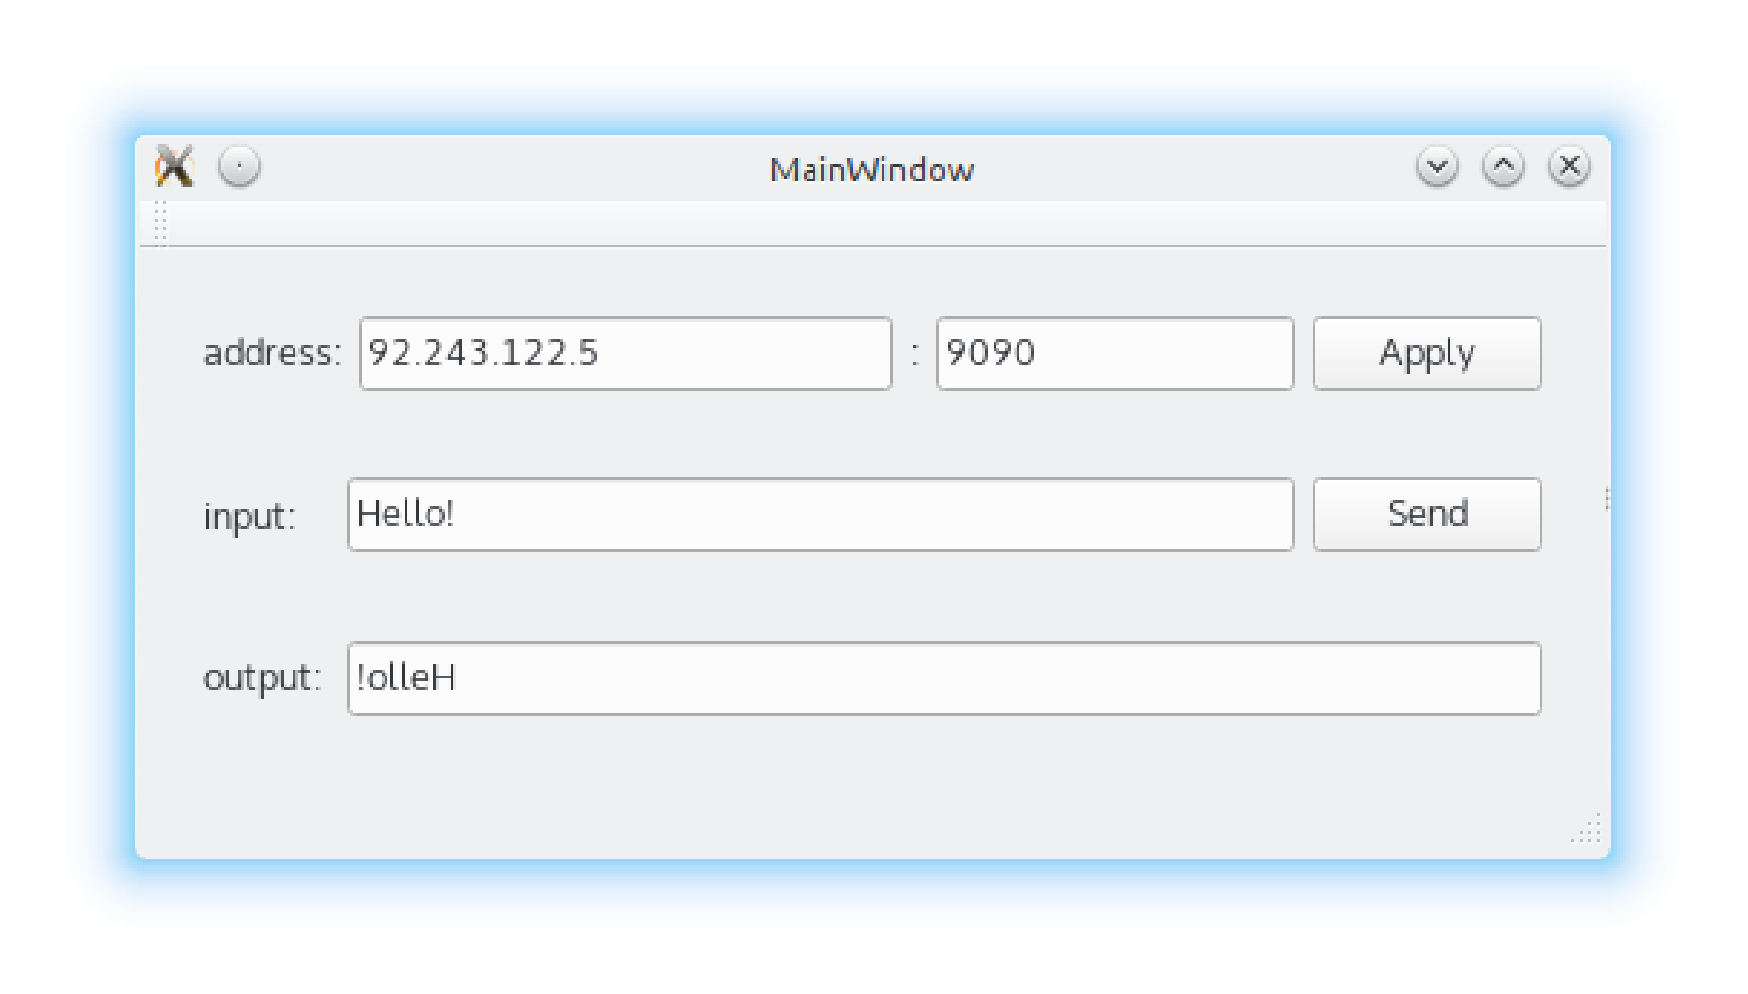
\includegraphics[width=0.8\linewidth]{window1}}
%  \caption{Подключение к эмулятору УСПД}
%  \label{window1:window1}
% \end{figure}

\subsection{Эмулятор ССД}

На сервере хранится список пользователей, которых поочередно опрашивает сервер. Данный список необходимо читать и редактировать.

Для решения данной задачи необходимо создать класс, описывающий объект-сервер, который будет хранить список клиентов и выполнять опрос клиентов.

На данный момент нет описания к системе команд УСПД, поэтому ограничимся передачей любого тестового сообщения клиенту при помощи реализованных ранее классов-сокетов.

Прототип класса-сервера представлен ниже:

\begin{lstlisting}
class MyServer : public QObject
{
    Q_OBJECT
public:
    explicit MyServer(QObject *parent = 0);
    ~MyServer();

    void addClient(const QString &name, 
		   const QString &addr, 
		   const int &port);
    QMap<QString, ClientAddress>* getClientsList();

private:
    QMap<QString, ClientAddress> clients;
    void timerEvent(QTimerEvent* event);
};
\end{lstlisting}

В конструкторе данного класса запускается таймер, которй отсчитывает интервалы времени между опросами списка клиентов. При обнулении таймера вызывается метод timerEvent в котором и происходит опрос списка клиентов, хранящегося в QMap<QString, ClientAddress>, ClientAddress - структура данных, хранящая ip-адрес и порт назначения.

Метод addClient принимает имея, ip-адрес и порт клиента, которого необходимо добавить в список и создает новый элемент в объекте clients.

getClientsList - метод, возвращающий атрибут clients.

timerEvent - метод, который просматривает список клиентов, для каждого клиента создает свое объект типа ClienSock(описан ранее), посылает клиенту массив байт, и отключается. 

Графический интерфейс программы представлен на рисунку \ref{server_gui:server_gui}.

\begin{figure}[ht!]
 \center{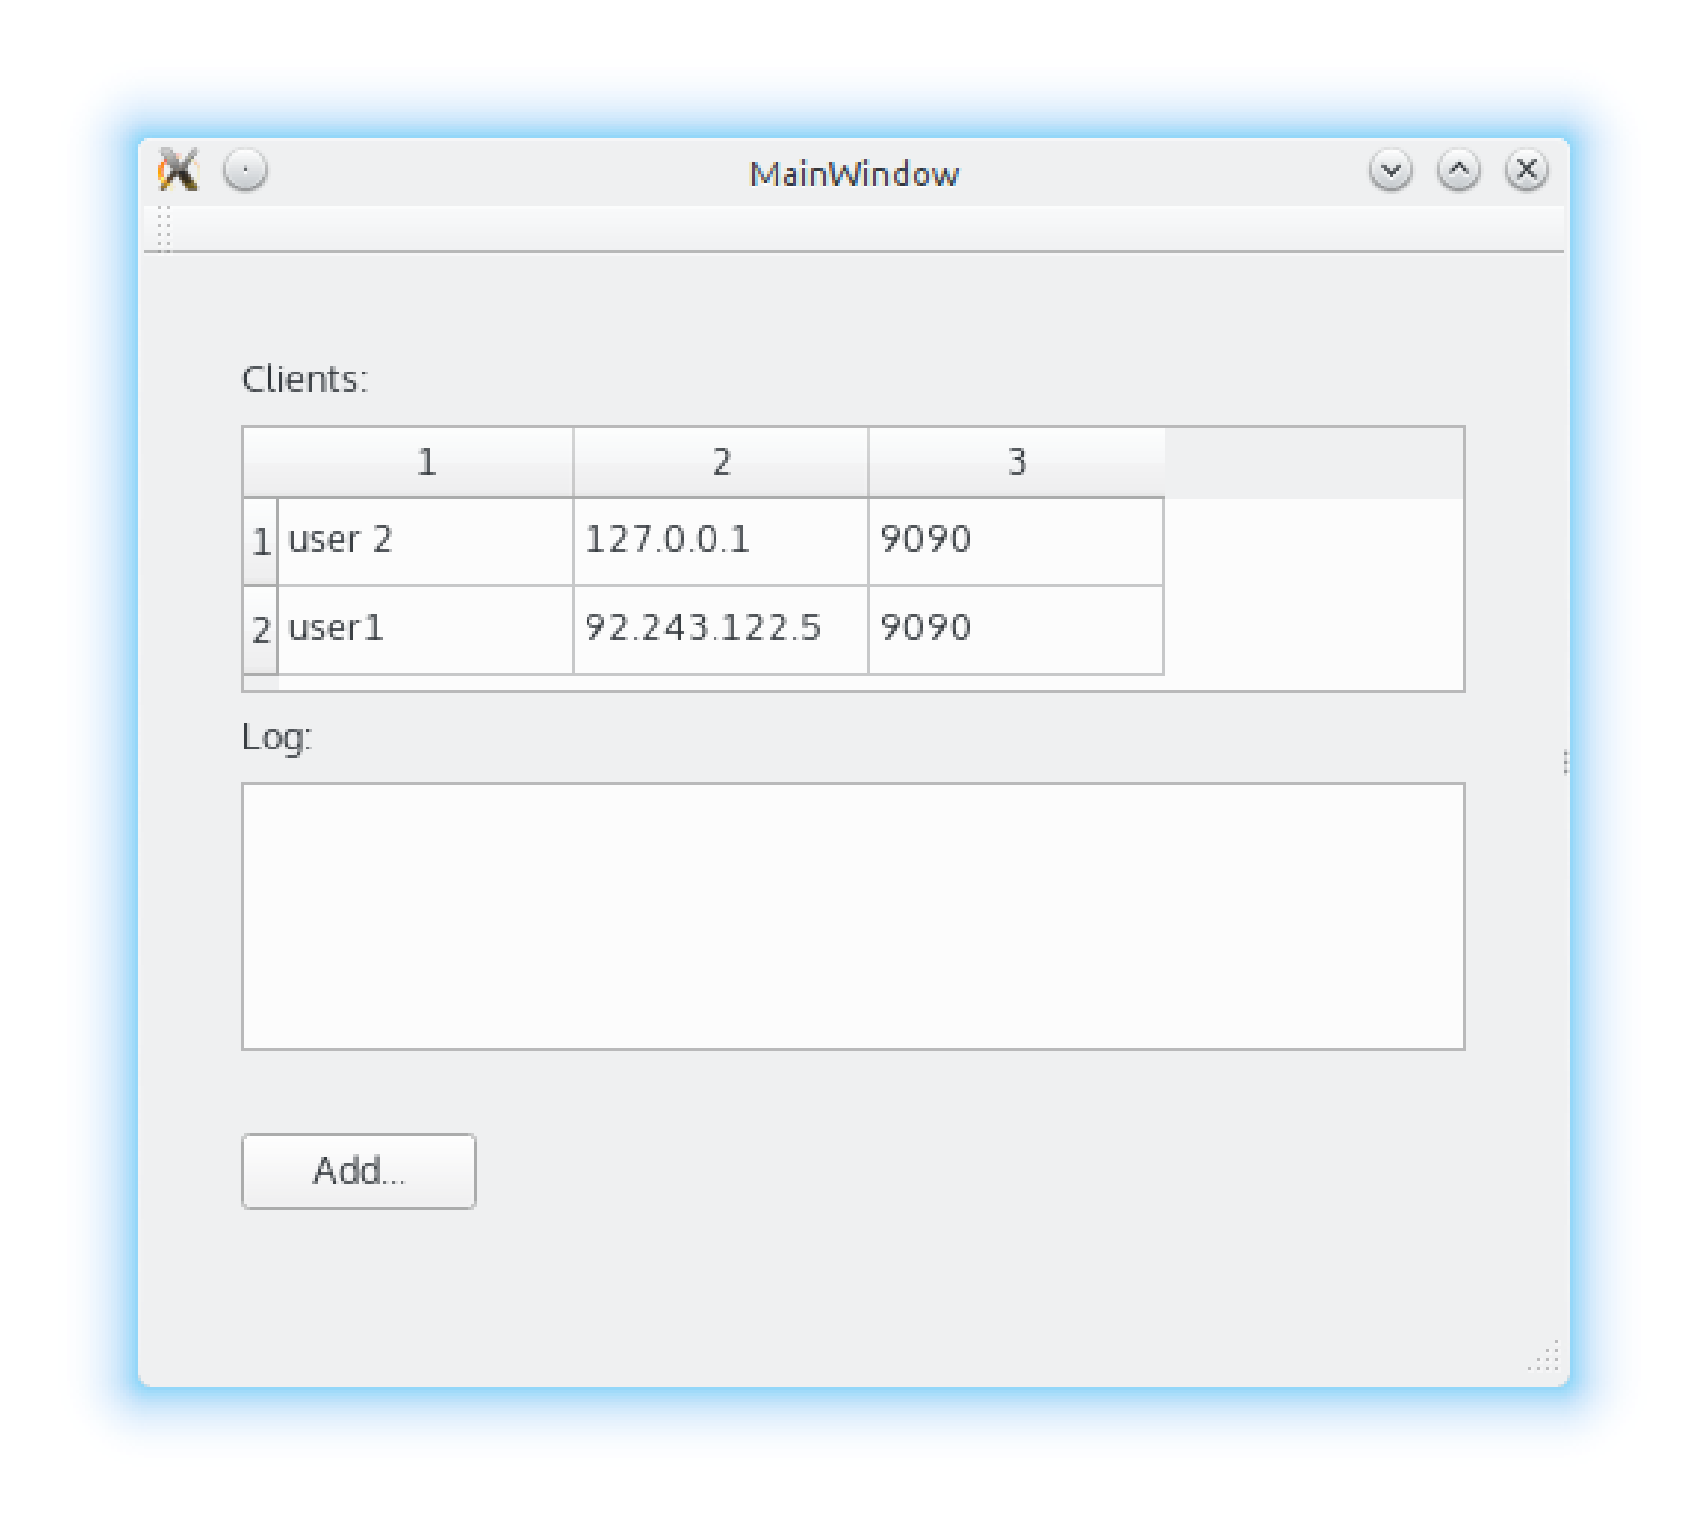
\includegraphics[width=0.7\linewidth]{server_gui}}
 \caption{Интерфейс программы}
 \label{server_gui:server_gui}
\end{figure}

Реакция эмулятора УСПД на user1 представлена на рисунке \ref{client_log:client_log}.

\begin{figure}[ht!]
 \center{\includegraphics[width=0.7\linewidth]{client_log}}
 \caption{Работа эмулятора УСПД}
 \label{client_log:client_log}
\end{figure}

\subsection{Проверка формирования пакетов}

Для тестирования работы протокола запустим эмулятор УСПД, после чего запустим эмулятор ССД и введем адрес УСПД. Запустим wireshark\cite{nix} и дождемся очередного цикла опроса. После чего восстановим TCP сессию и рассмотрим структуру ответа. Структура ответа представлена на рисунке \ref{img:test_pachete}.

\begin{figure}[ht!]
 \center{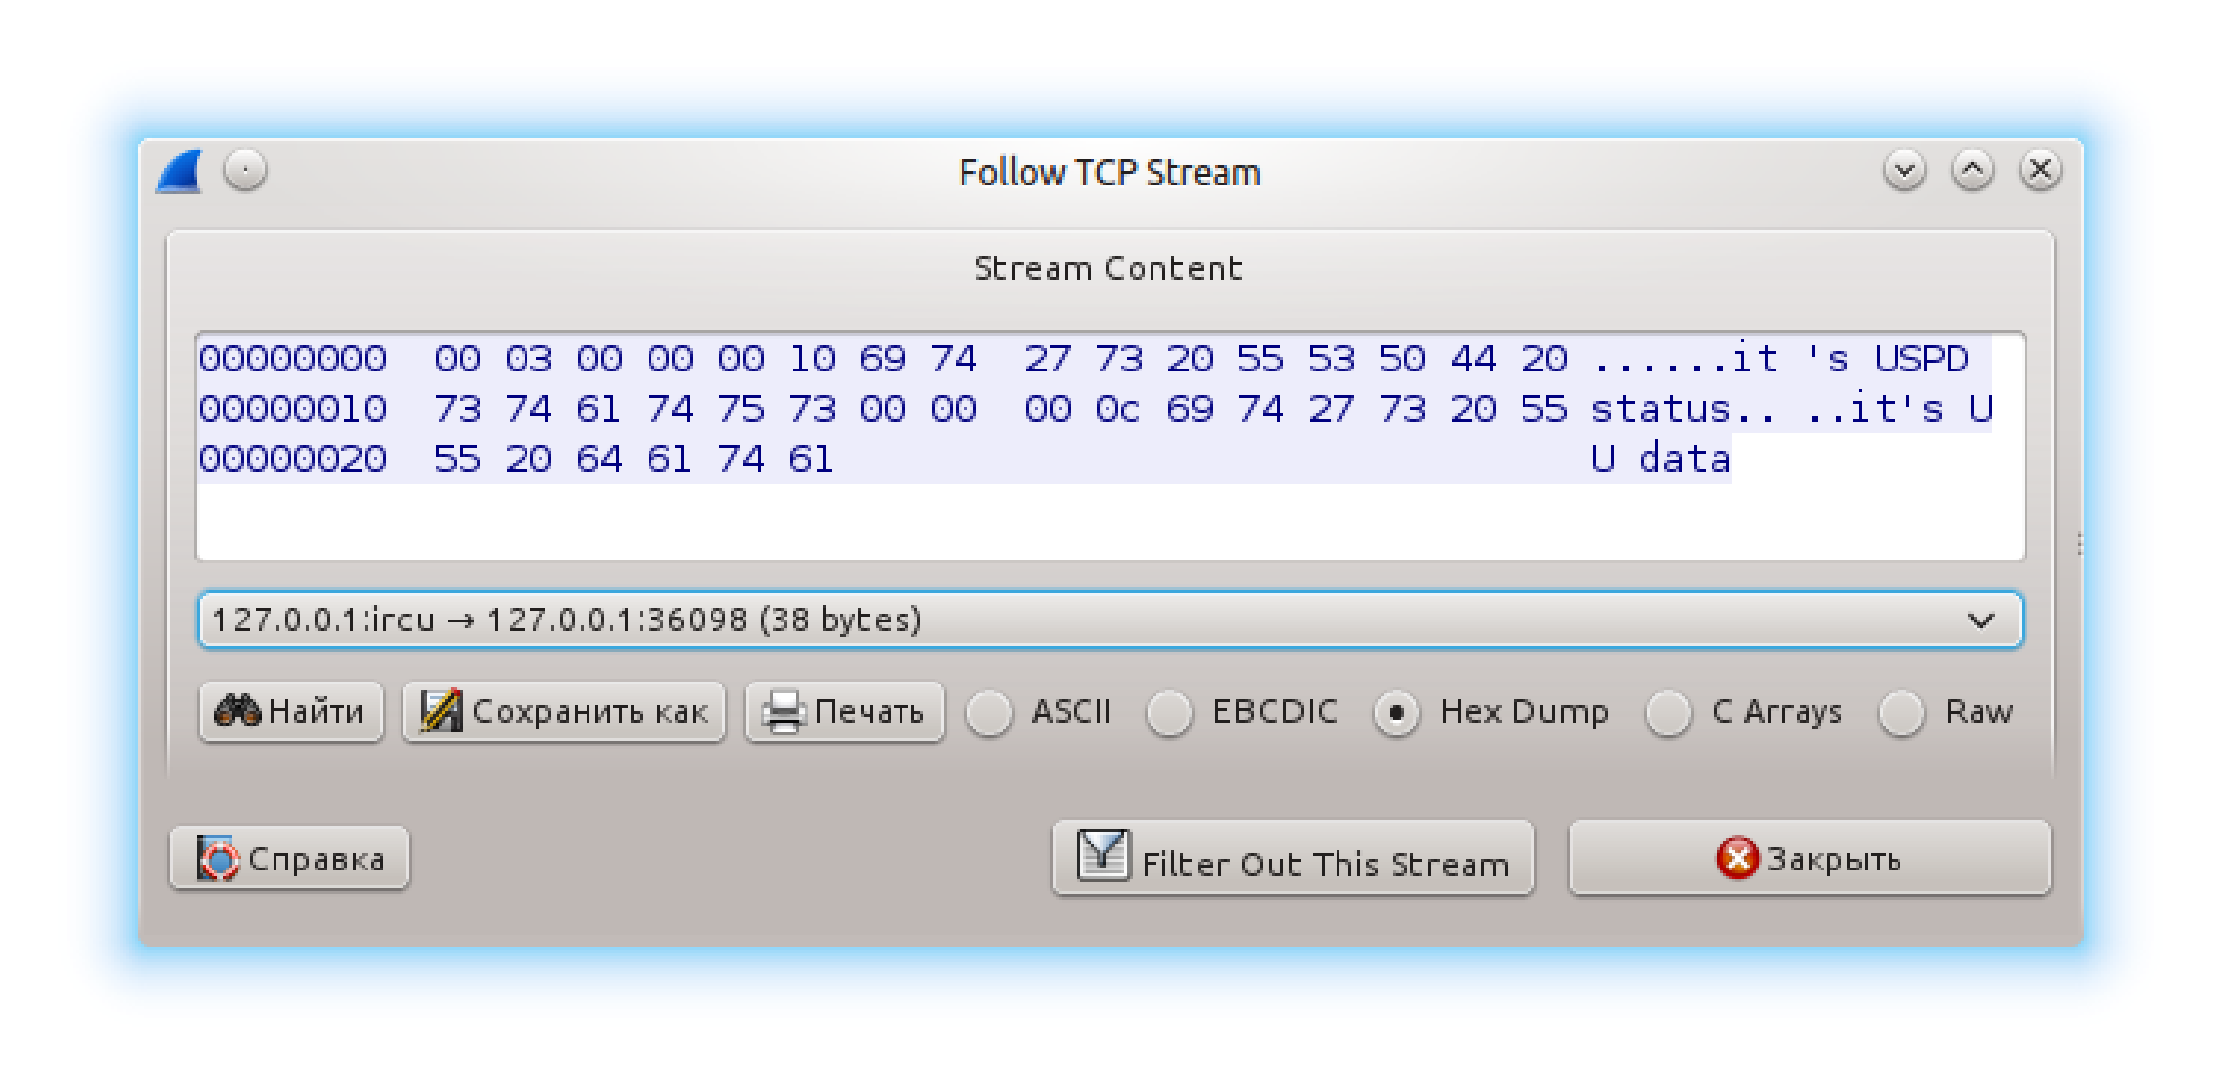
\includegraphics[width=0.7\linewidth]{test_pachete}}
 \caption{Ответ УСПД}
 \label{img:test_pachete}
\end{figure}

На рисунке представлена часть с ответом УСПД восстановленной TCP-сессии между эмуляторами. Разберем структура по байтам:

\begin{itemize}
 \item 00 03 - первые два байта, двухбайтовый ID УСПД. Совпадает с тестовыми данными УСПД;
 \item 00 00 00 10 - 4 байта - размер блока информации о состоянии УСПД. Равен 16;
 \item На рисунке видно что следующие 16 байт составляют строку состояния УСПД указанную в эмуляторе;
 \item 00 00 00 0с - 4 байта - размер блока информации от устройств учетаю Равен 12;
 \item На рисунке видно что следующие 12 байт составляют строку данных УУ указанную в эмуляторе.
\end{itemize}

На основании разбора можно сделать вывод что сформированный пакет совпадает со структурой пакета, описанной в разделе ``выходные данные''. % тестирование
 \section{Система команд УСПД}

Все команды можно разбить на группы:

\begin{itemize}
 \item регистрационные;
 \item настройка;
 \item запроса данных;
 \item запроса статуса;
 \item отладочные;
 \item управления.
\end{itemize}

\subsection{Команды регистрации на УСПД}

Данные команды отвечают за процедуры идентификации и аутентификации пользователя на УСПД. Перечень команд представлен в таблице \ref{tab:ident_comand}.

\begin{center}
 \begin{longtable}[h]{|*3{p{5cm}|}}
  \caption{Команды идентификации} \label{tab:ident_comand} \\
  \hline
  Команда & описание & формат \\
  \hline
  \endfirsthead
  регистрация в системе & передача имени пользователя и начало процедуры авторизации & login user\_name \\
  \hline
  завершение сеанса & завершение работы пользователя и выход из системы & logout \\
  \hline
 \end{longtable}
\end{center}


%TODO

\subsection{Команды настройки УСПД}

Данные команды предназначены для настройки УСПД и подконтрольных ему счетчиков. Присвоения идентификаторов, установки интервала опроса счетчиков, разграничения доступа к функционалу. Перечень команд представлен в таблице \ref{tab:config_comand}.

\begin{center}
 \begin{longtable}[h]{|*3{p{5cm}|}}
  \caption{Команды настройки УСПД} \label{tab:config_comand} \\
  \hline
  Команда & описание & формат \\
  \hline
  \endfirsthead
  конфигурация системы & производится поиск подключенных датчиков, присвоение им id и вывод информации о проделанной работе & configure \\
  \hline
  установка времени & устанавливает системное время & set\_time value \\
  \hline
 \end{longtable}
\end{center}

%TODO

\subsection{Команды получения данных от УСПД}

Данные команды используются для получения информации от счетчика или их группы. Перечень команд представлен в таблице \ref{tab:gd_comand}. 

\begin{center}
 \begin{longtable}[h]{|*3{p{5cm}|}}
  \caption{Команды управления дынными} \label{tab:gd_comand} \\
  \hline
  Команда & описание & формат \\
  \hline
  \endfirsthead
  получение данных от счетчиков & отправляет запрос данных с указанного счетчика & get\_data device\_id \\
  \hline
 \end{longtable}
\end{center}

%TODO

\subsection{Команды получения статуса УСПД}

Данные команды используются для получения информации о состоянии УСПД и подконтрольных ему счетчиков. Перечень команд представлен в таблице \ref{tab:gs_comand}.

\begin{center}
 \begin{longtable}[h]{|*3{p{5cm}|}}
  \caption{Команды получения системной информации} \label{tab:gs_comand} \\
  \hline
  Команда & описание & формат \\
  \hline
  \endfirsthead
  получение информации о состоянии системы & Получение значения времени, количества счетчиков, времени последнего сеанса передачи даных & get\_sys\_info \\
  \hline
  получение списка идентификаторов счетчиков & Возвращает список device\_id всех подконтрольных счетчиков & get\_devices\_list \\
  \hline
  получить сведения о состоянии счетчика & получить статус указанного счетчика & get\_sensore\_status \\
  \hline
  системное время & возвращает текущее значение времени на УСПД & get\_time \\
  \hline
 \end{longtable}
\end{center}

%TODO

\subsection{Команды отладки УСПД}

Данные команды предназначены для разработчиков и помогают отлаживать систему. Перечень команд представлен в таблице \ref{tab:debug_comand}.

\begin{center}
 \begin{longtable}[h]{|*3{p{5cm}|}}
  \caption{Отладочные команды} \label{tab:debug_comand} \\
  \hline
  Команда & описание & формат \\
  \hline
  \endfirsthead
  установить значения счетчика & указывает, какие данные должен вернуть счетчик при следующем его опросе & set\_data device\_id data \\
  \hline
 \end{longtable}
\end{center}

%TODO

\subsection{Команды управления УСПД}

Команды перезагрузки, сброса настроек и прочее. Перечень команд представлен в таблице \ref{tab:sys_comand}.

\begin{center}
 \begin{longtable}[h]{|*3{p{5cm}|}}
  \caption{Системные команды} \label{tab:sys_comand} \\
  \hline
  Команда & описание & формат \\
  \hline
  \endfirsthead
  перезагрузка устройства & перезагружает систему & restart \\
  \hline
 \end{longtable}
\end{center}

%TODO
 
 \newpage
 \section*{Список использованных источников}
 \addcontentsline{toc}{section}{Список использованных источников}
 1. РБК Research. Энергосбережение: приборы учета [Электронный ресурс] - URL: http://marketing.rbc.ru/research/562949989113292.shtml. (Дата обращения: 20.02.2015).
 
 2. Обзор и варианты построения архитектуры АСКУЭ // цсп ТУСУР. - 2014.
 
 3. Шлее, М. Qt 4.5: Профессиональное программирование на С++ / Макс Шлее. - СПб.: БХВ Петербург, 2010. - 896 с.
 
 4. Дуглас Камер. Сети TCP/IP, том 1. Принципы, протоколы и структура = Internetworking with TCP/IP, Vol. 1: Principles, Protocols and Architecture. — М.: «Вильямс», 2003. — С. 880. — ISBN 0-13-018380-6.
 
 5. Иванов М. А. Криптографические методы защиты информации в компьютерных системах и сетях. — М.: КУДИЦ-ОБРАЗ, 2001. — 368 с.
 
 6. Михаэль Кофлер. Linux. Установка, настройка, администрирование. - Питер, 2014. - 768 c.
 
 7. Безопасность жизнедеятельности. Учебное пособие. Смирнов Г.В., Кодолова Л.И. – Томск. ТУСУР 2007
 
 8. СанПиН 2.2.2/2.4.1340-03 ``Гигиенические требования ПЭВМ и организации работы на них''
 
 9. ТОИ Р-45-084-01 ``Типовая инструкция по охране труда при работе на персональном компьютере''
\end{document}
